% !TEX root = ../main.tex

\chapter{State of the art} \label{chap:state-of-the-art}

This chapter defines the concept of machine learning and presents a comprehensive overview of the most relevant algorithms and models.

\section{Machine learning} \label{sec:machine_learning}


The term \textit{Machine Learning} (ML) first appeared in the late 50's in the field of computer science and now it is becoming a buzzword used in several contexts spanning from particle physics and astronomy to medicine and social sciences~\cite{service2017ai}.
With a simple search on Google Trends\footnote{\url{https://trends.google.com}} it is possible to roughly quantify the pervasiveness of this term on the Internet in the last few years. From Figure~\ref{fig:google_trend_ML} we can see that the interest toward both the terms \textit{machine learning} and \textit{data science} are growing, with the first consistently superior to the second.

\begin{figure}[h!]
  \centering
    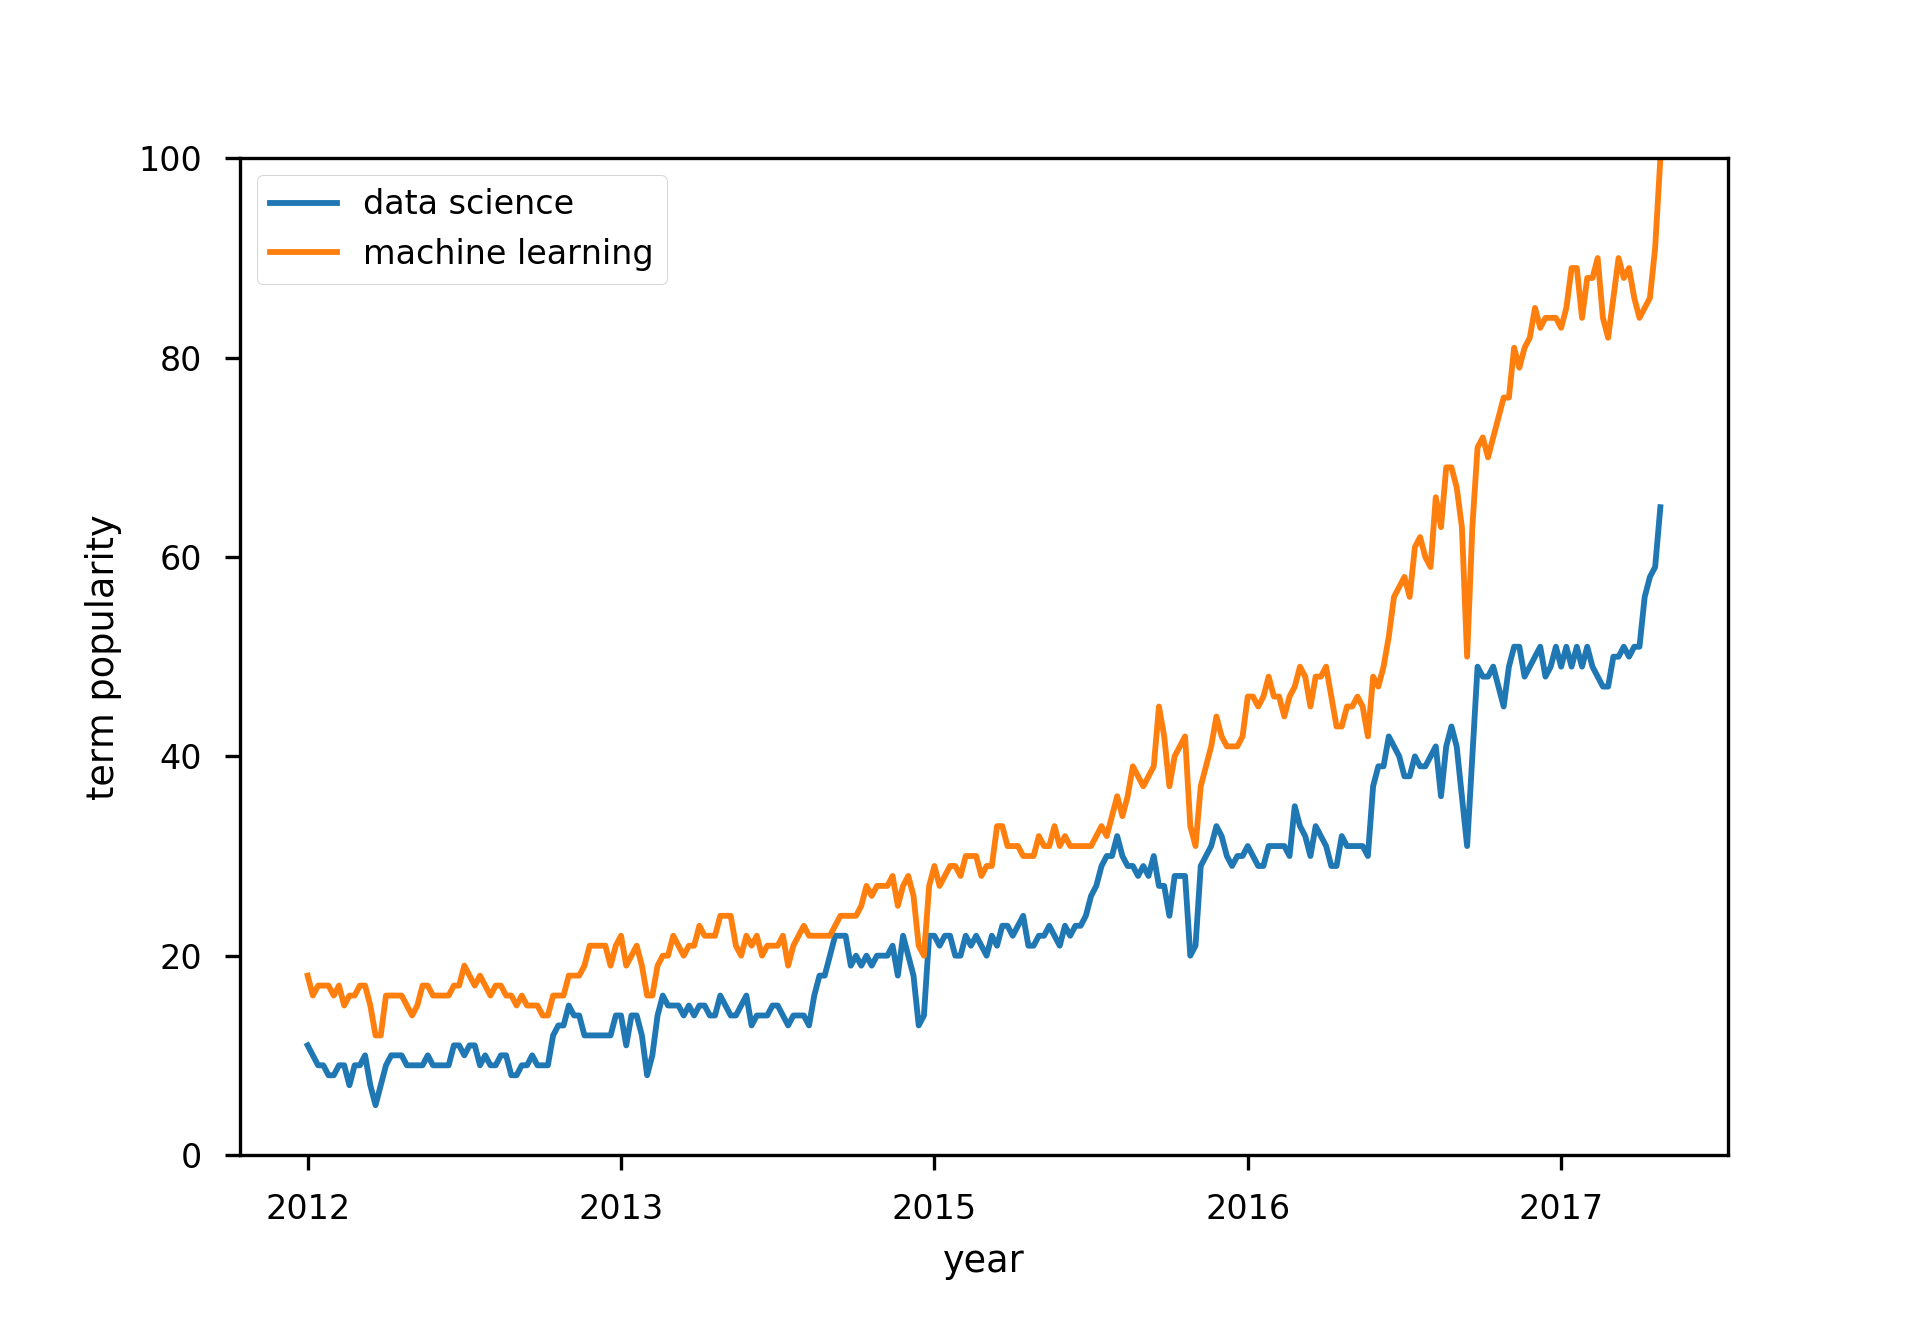
\includegraphics[width=0.8\textwidth]{part1/google_trends_MLDS.png}
  \caption{The Internet popularity over the past five years of two terms: \textit{data science} and \textit{machine learning}. The vertical axis represents a normalized measure of the number of Google search query of an input term. The trend is normalized with respect to its maximum (source: Google Trends).} \label{fig:google_trend_ML}
\end{figure}

A possible explanation to this phenomenon can be found in a recent article published on Science~\cite{appenzeller2017revolution} in which the authors describe a new \textit{scientific revolution} lead by an explosion in the modern data collection abilities.
Such massive amounts of data have long overwhelmed human analysis and insights potential and this makes ML a key element for scientists trying to make sense of large-scale observations.

But, what is \textit{machine learning}? And how does it differ from statistics?

A unique answer to this question may not be easy to provide. In fact, ML can be defined in different ways and from several standpoints. Let's see three remarkable examples.

\begin{enumerate}
  \item Kevin P. Murphy in its \emph{Machine Learning - A Probabilistic Perspective}~\cite{murphy2012machine} defines machine learning as follows.

  \begin{displayquote}
  "[...] \emph{a set of methods that can automatically detect patterns in data, and then use the uncovered patterns to predict future data, or to perform other kinds of decision making under uncertainty} [...]"
  \end{displayquote}

  \item Trevor Hastie, a well-known applied statistician, in a famous seminar\footnote{part of Data Science @ Stanford Seminar series (source: \url{https://goo.gl/UFgqxU}).}, held in October 2015 at the Stanford University, gave the following three definitions.

  \begin{displayquote}
    \begin{itemize}
      \item[] \emph{{\bf Machine Learning} constructs algorithms that can learn from data.}
      \item[] \emph{{\bf Statistical Learning}  is a branch of applied statistics that emerged in response to machine learning, emphasizing statistical models and assessment of uncertainty.}
      \item[] \emph{{\bf Data Science}  is the extraction of knowledge from data, using ideas from mathematics, statistics, machine learning, computer science, engineering...}
    \end{itemize}
  \end{displayquote}

  \item Carl E. Rasmussen in the preface of its \emph{Gaussian Processes for Machine Learning}~\cite{rasmussen2006gaussian} introduces the difference between statistics and ML as follows.

  \begin{displayquote}
    "\emph{in statistics a prime focus is often in understanding the data and relationships in terms of models giving approximate summaries such as linear relations or independencies. In contrast, the goals in machine learning are primarily to make predictions as accurately as possible and to understand the behaviour of learning algorithms}"
  \end{displayquote}

\end{enumerate}

It looks like each author, according to his background, expertise and experiences, provides a slightly different definition of ML. Trying to summarize these three standpoints, we can say that \emph{ML is an interdisciplinary field that borrows the concept of data-driven model from statistics in order to devise algorithms that can exploit hidden patterns in current data and make accurate predictions on future data}.

As of today ML is the workhorse of data science.


  \subsection{Supervised learning} \label{subsec:supervised_learning}

  Humans are remarkably good at \emph{learning by examples}. When a kid is taught what a pencil looks like, he will be capable of understanding the concept of pencil from a limited number of guided observations. Similarly, when future radiologists are trained to distinguish between healthy tissues from tumors in MRI scans, they will be provided with several annotated biomedical images from which they will be able to generalize.
  This learning paradigm is characterized by the presence of two key objects: \textit{data} and \textit{labels}. In the last example, we will consider the MRI scans as data, and their annotations (\eg tumor vs healthy tissue) as labels.

  Supervised learning is the branch of ML, in which predictive models are trained on labeled data. In the ML jargon, and in this thesis, one usually refers to data as collections of \textit{samples} described by an arbitrarily large number of \textit{predictors} (or \textit{features}) that are used as \textit{input} in the training process having labels as its \textit{otput}.

  In general, input samples $x$ throughout this thesis are represented as $d$-dimensional vectors in an input space $\mathcal{X}$, where $\mathcal{X}\subseteq\mathbb{R}^d$, while the labels $y\in\mathcal{Y}$. The nature of the output space $\mathcal{Y}$ defines the learning task as \textit{binary classification} if  $\mathcal{Y} = \{-1,+1\}$, \textit{multiclass classification} if $\mathcal{Y} = \{1,2,\dots,k\}$,
  \textit{regression} if $\mathcal{Y}\subseteq\mathds{R}$ and
  \textit{vector-valued regression} if $\mathcal{Y}\subseteq\mathds{R}^k$.
  Each one of these learning problems will be faced in the second part of the thesis and for each problem a possible data-driven solution will be proposed. The remainder of this section describes the methods that are most relevant with the adopted models and pipelines.


    \subsubsection{Regularization methods}
    % rubare da BIB
    % In its most classical definition, the aim of modeling is to infer some unknown structure underlying the data.
    The process of identifying a model from a real-world data collection can be very hard. Many unwanted and concurrent factors may be misleading and the result may have poor predictive power. For instance, the acquisition devices may introduce random fluctuations in the measures or the amount of collected samples $n$ may be small with respect to the number of observed variables $d$ which, in turn, may not even be representative of the target phenomenon. From a modeling standpoint, every combination of the factors above can be seen as \textit{noise} affecting the data.
    Precautions in the model formulation process must be taken in order to achieve solutions that are \textit{robust} to the noise effect.

    In the field of ML, a common strategy to build predictive models out of noisy data is called \textit{regularization}. As the biomedical world is the the main area of interest of this Thesis (see Section~\ref{sec:challenges_biomedical}), on each learning algorithm described, particular emphasis will be put on the relevant regularization strategies.

    In its broader definition regularization is the process of introducing additional information in order to solve a possibly ill-posed problem \cite{tikhonov1963solution, evgeniou2000regularization}. The expected result is a function that fits the training data while having good generalization properties, \ie accurate predictions on previously  \textit{unseen} test data \cite{hastie2009elements}. In ML, a model that fits well the training data but performs poorly on new samples is said to be \textit{overfitting} the training set.

    Given a set of input-output pairs $\{X, Y\}$, the main objective of {\em supervised learning} is to find a function of the inputs $f(X)$ that approximates the outputs $Y$. This translates into the minimization problem defined in Equation~\eqref{eq:losspen}.

    \begin{equation}\label{eq:losspen}
    	\min_f \frac{1}{n}\sum_{i=1}^n V(f(\bm{x}_i),y_i) + \lambda R(f)
    \end{equation}

    The loss function $V(\cdot,\cdot)$ can be seen as a measure of \textit{adherence} to the available training data. Several loss function for regression and classification problems were proposed; in Table~\ref{tab:losses} we define the most commonly adopted in biomedical studies and their visual representation is presented in Figure~\ref{fig:loss}. The regularization penalty $R(\cdot)$ imposes stability on the expected function exploiting the available prior knowledge on the problem~\cite{tikhonov1963solution}.

    \begin{figure}[!ht]
        \centering
        \subfloat[]{%
            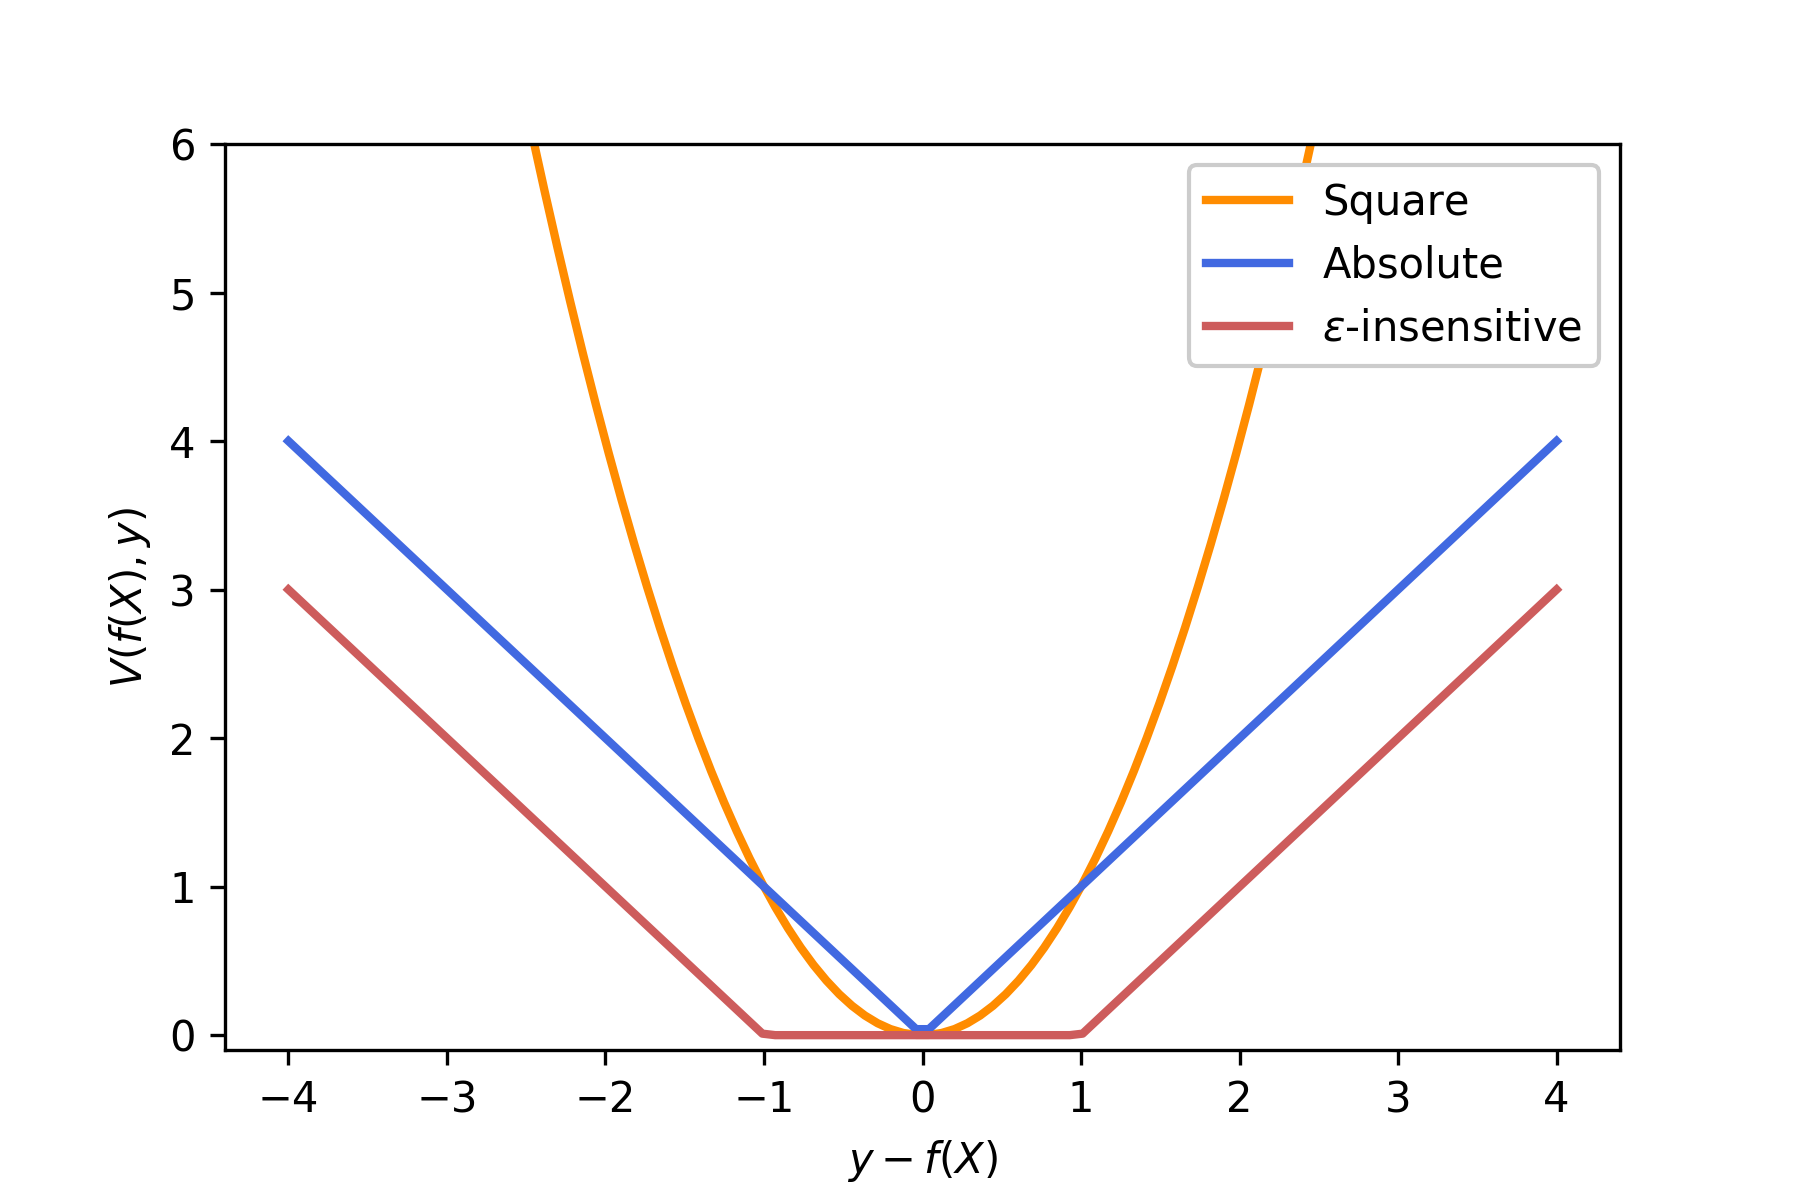
\includegraphics[width=0.5\textwidth]{part1/regression_losses.png}
            \label{fig:regression}%
        }%
        % \hfill%
        \subfloat[]{%
        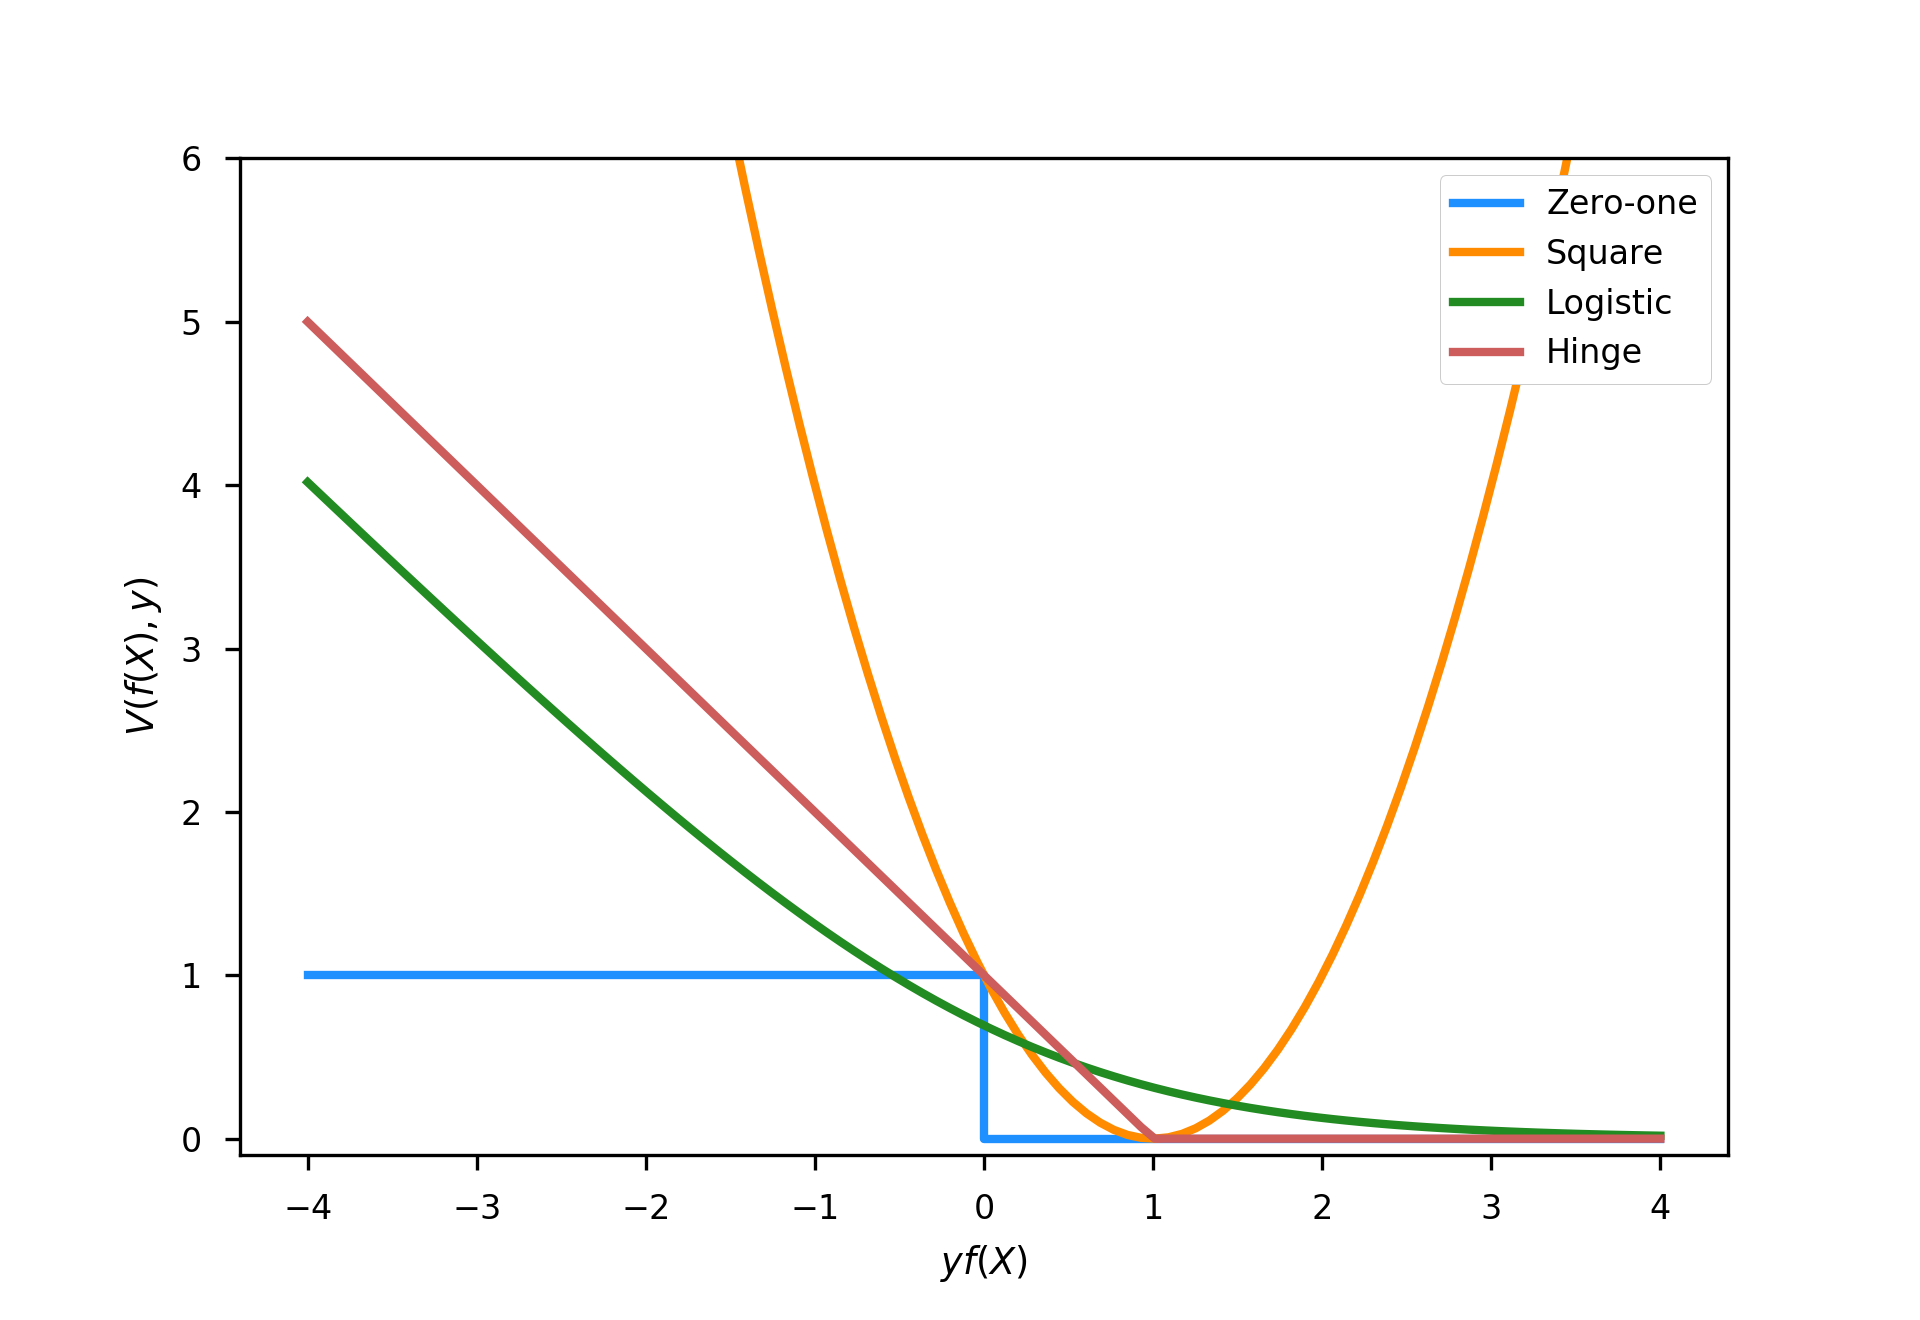
\includegraphics[width=0.5\textwidth]{part1/classification_losses.png} \label{fig:classification}
        }%
        \caption{An overview on the most common loss functions for regression (a) and classification (b) problems plotted against the corresponding prediction error.}\label{fig:loss}
    \end{figure}


    \begin{table}[]
      \centering
      \caption{Definition of the loss functions for regression (top) and classification (bottom) problems represented in Figure~\ref{fig:loss}.}\label{tab:losses}
      \begin{tabular}{@{}ll@{}ll@{}}
        \toprule
        Loss function & $V(f(\bm{x}),y)$  & Learning problem           \\ \midrule
        Square                   & $(y - f(\bm{x}))^2$ & regression \\
        Absolute                 & $|y - f(\bm{x})|$ & regression   \\
        $\epsilon$-insensitive   & $\begin{cases}
            0 & \text{if } |y-f(\bm{x})| < \epsilon\\
            |y-f(\bm{x})| - \epsilon & \text{otherwise}
        \end{cases} $        & regression                 \\
        \midrule
        Zero-one               & $\begin{cases}
            0 & \text{if } y = f(\bm{x})\\
            1 & \text{otherwise}
        		\end{cases}$ & classification \\
        Square                 & $(1 - yf(\bm{x}))^2$ & classification  \\
        Logistic                 & $\log(1 + e^{-yf(\bm{x})})$ & classification  \\
        Hinge                 & $|1 - yf(\bm{x})|_+$ & classification  \\
        \bottomrule
      \end{tabular}
    \end{table}


    \subsubsection{Ensemble methods}
    \subsubsection{Deep learning}


  \subsection{Unsupervised learning} \label{subsec:unsupervised_learning}
    \subsubsection{Manifold learning}
    \subsubsection{Clustering}


  \subsection{Model selection and evalutation} \label{subsec:model_selection}
    \subsubsection{Model selection strategies}
    % cross validation flavours
    \subsubsection{Feature selection stability}
    % stability selection
    \subsubsection{Performance metrics}
    % sup and unsup
    % acc, f1, mcc, ...


\section{Computational requirements and implementations} \label{sec:implementation}
\begin{itemize}
  \item MPI
  \item GPU and accelerators
\end{itemize}
